\documentclass{article}
\usepackage[utf8]{inputenc}
\usepackage{amsmath}
\usepackage{graphicx,float}
\usepackage{enumerate}
\usepackage{amssymb}
\usepackage[a4paper,
            bindingoffset=0.2in,
            left=1in,
            right=1in,
            top=1in,
            bottom=1in,
            footskip=.25in]{geometry}
            

\title{CS 754 Project Report  \\ Robust video denoising using Low rank matrix completion}
\author{Piyush Bharambe(18D070019) \\
Vinit Awale(18D070067)}
\date{May 2022}

\begin{document}

\maketitle

\section{Introduction}
Video denoising is different from image denoising because video sequences have high temporal redundancies which can be exploited for better results. Most methods are based on a single statistical model (eg heavy gaussian noise) and so perform poor in presence of other noise as well.

In this report, we present the method for video denoising introduced by H. Ji et.al \cite{H Ji}. The method uses low rank matrix completion for patch based denoising to remove mixed noise from video data.
We implemented this method and got results consistent with that of the authors.  

\section{Problem statement}
We are given $\mathcal{F} = \{f_k\}_{k=1}^K$, a image sequence with K frames. Each image $f_k$ is sum of its underlying clean image $g_k$ and noise $n_k$
\begin{equation*}\label{eq1}
    f_k = g_k + n_k
\end{equation*}

The goal is to recover $\mathcal{G} = \{g_k\}_{k=1}^K$ by removing $n_k$ from $f_k$. Here noise $n_k = n_k^g+ n_k^p +n_k^i$, i.e. sum of gaussian, poisson and impulsive noise. $n_k^g - \mathcal{N}(0, \sigma^2 I)$ (amplifier noise) , $n_k^p$ is poisson noise (shot noise) with zero mean and varaince $\kappa$, $n_k^i$ is impulsive noise with parameter $s$ (by dead pixels, converter or transmission errors)

\section{Methodology}
Consider a patch $p_{j,k}$ of size $n \times n \times c$(here c = no. of channels). Taking this as a reference patch we search for m similar patches in both the temporal and spatial neighbourhood.  Vectorize each patch in to a column and concatenate those columns to find a $n^2c \times m$ patch matrix $P_{j,k}$. Then we can rewrite our problem \ref{eq1} as 
\begin{equation*}
    P_{j,k} = Q_{j,k}+N_{j,k}
\end{equation*}

In first stage of algorithm, we do patch match and find the patch matrix as stated above. Then we find the reliable elements of the patch matrix $P_{j,k}$ which are identified based on deviation from mean of each row and the adaptive median filter based impulsive noise detector. Let $\Omega$ be set of all such reliable pixels. 

In second stage, we recover $Q_{j,k}$ from the incomplete version of $P_{j,k}$ denoted by $P_{j,k}|_{\Omega}$. This is done using low rank completion methods. We have used the fixed point iteration algorithm for it. 


\subsection{Patch matching and grouping}
First we perform adaptive median filtering by the RAMF (Rank order based adaptive median filtering) method \cite{median} to remove the impulsive noise which can affect the patch matching severely. The RAMF method involves two stages- in first stage, we increase the window size till the median filter output is not corrupted, and in second stage, if the central pixel is corrupted, we replace it with median filter output else we leave it as it is. RAMF works best for detecting and removing positive and negative impulse noise.

We use an exhaustive search algorithm for finding similar patches. For measuring similarity, we use the mean absolute difference between patches. We search within a predefined neighbourhood of the frame of reference patch and within a predefined temporal neighbourhood. (in our case, we used 20x20 spatial neighbourhood and a temporal neighbourhood size of 5 frames.) We collect best p similar patches within each frame. Then we vectorize all patches by concatenating columns to get a single column vector. All vectorized patches are then concatenated to get the patch matrix. 

The index set $\Omega$ includes all reliables points in the patch matrix. We first identify the corrupted pixels by the impulsive noise detector in the adaptive median filtering applied earlier. Next we identify pixels which deviate more than a predefined threshold from the mean of the row of the patch matrix. $\Omega$ is then calculated by including all pixels except the aforementioned two types of corrupted/unreliable points. After this we perform the low rank matrix completion.


\subsection{Low rank matrix completion}
$Q_{j,k}$ is recovered from $P_{j,k}|_{\Omega}$ by solving the minimization problem,
\begin{equation*}
    \min_{Q} ||Q||_{*} \text{ } s.t. \text{ } ||Q|_{\Omega} - P|_{\Omega}||_F^2  < \#(\Omega) \hat{\sigma}^2
\end{equation*}

where $||.||_F$ is the Frobenius norm and $\hat{\sigma}$ is the estimated standard deviation of noise which is obtained by calculating the average of the variances of all elements $\in \Omega$ on each row.
$\#(\Omega)$ is the cardinality of set $\Omega$. $P|_{\Omega}$ denotes matrix including elements with indices in $\Omega$ omly

We solve its Lagrangian version 
\begin{equation*}
    \min_{Q} \frac{1}{2} ||Q|_{\Omega} - P|_{\Omega}||_F^2 + \mu ||Q||_{*}
\end{equation*}

Here $\mu$ is chosen as $\mu = (\sqrt{n_1} + \sqrt{n_2})\sqrt{p}\hat{\sigma}$ where $n_1 \times n_2$ is the patch matrix size (in our case $n_1 = n^2c, n_2=m$) and p is ratio of number of pixels in $\Omega$ over number of pixels in patch matrix. 

Let the SVD of X be $X = U\Sigma V^T$. Then the soft shrinkage operator $D_\tau (X)$ is defined as 
\begin{equation*}
    D_{\tau}(X) = U\Sigma_{\tau} V^T
\end{equation*}
where $\Sigma_{\tau} = diag(max(\sigma_i - \tau, 0))$.

Now we use the following fixed iteration algorithm \cite{svt} for solving the minimization problem:

\begin{center}
    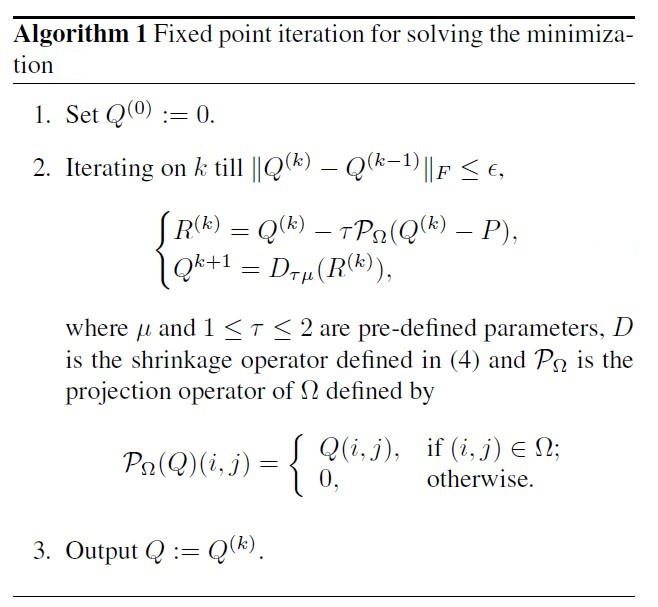
\includegraphics[scale=0.6]{algo.jpg}
\end{center}



\section{Experiments settings}
We set patch size as $8 \times 8 \times 3$ for RGB images. Number of frames = 20. Threshold for finding $\hat{\sigma}$ = 50. Patch search region around reference patch = $20 \times 20 \times 3$. We find 5 best similar patches per frame across 10 neighbour frames. We take strides of 4. Max window size for median filtering is 6. Step size for SVT = 1.5 

Taking above parameter values, we simulate for different values of noise parameters ($\sigma , \kappa, s$ ). The results are in next section.

\newpage
\section{Results}
\subsection*{Bus Data}
\subsubsection*{Gaussian dominated noise}
The noise parameters used are: \\
\begin{itemize}
    \item $\sigma = 50$
    \item $\kappa = 15$
    \item $s = 0.2$
\end{itemize}

\begin{figure}[H]
    \centering
    \begin{minipage}{.45\textwidth}
        \centering
        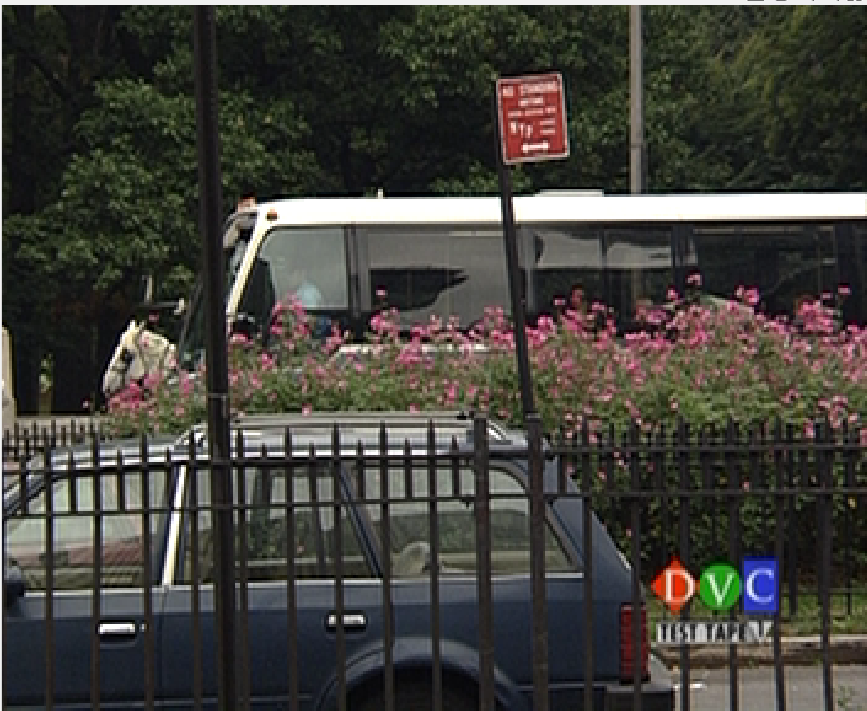
\includegraphics[width=\linewidth]{Images/Bus_original.png}
        \caption{Original Video frame}
        \label{fig:totalpowervst}
    \end{minipage}
    \begin{minipage}{.45\textwidth}
        \centering
        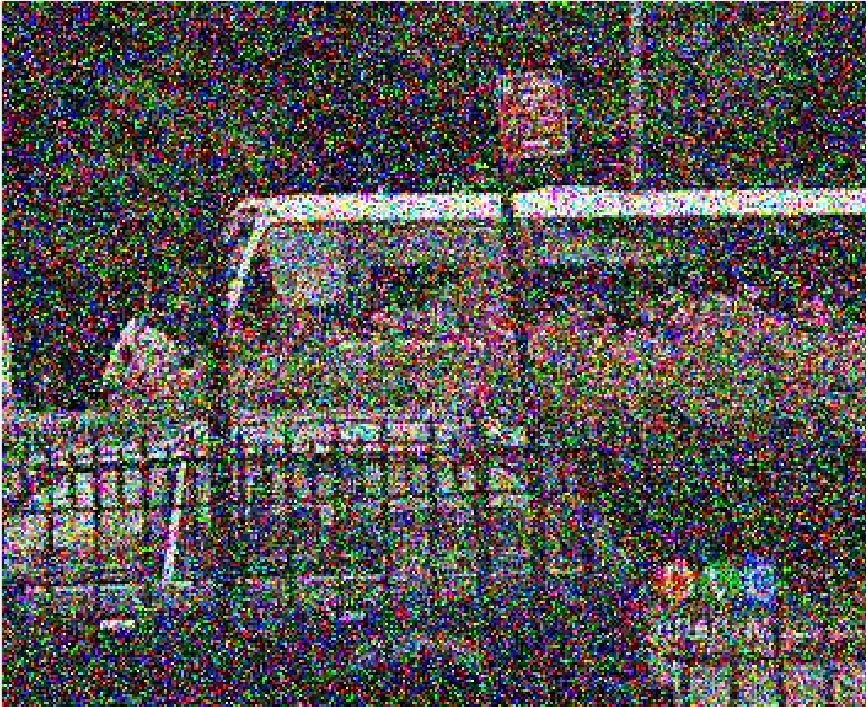
\includegraphics[width=\linewidth]{Images/Bus_1_noisy.png}
        \caption{Noisy Video frame}
    \end{minipage}
\end{figure}
\begin{figure}[H]
    \centering
    \begin{minipage}{.45\textwidth}
        \centering
        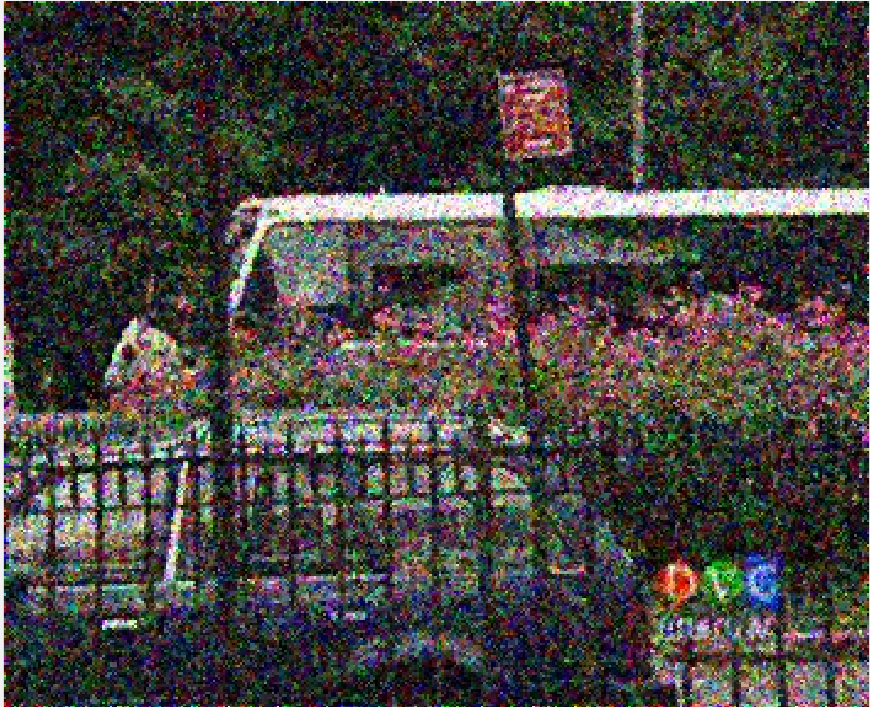
\includegraphics[width=\linewidth]{Images/Bus_1_median_filter.png}
        \caption{Result of Median Filtering}
    \end{minipage}
    \begin{minipage}{.45\textwidth}
        \centering
        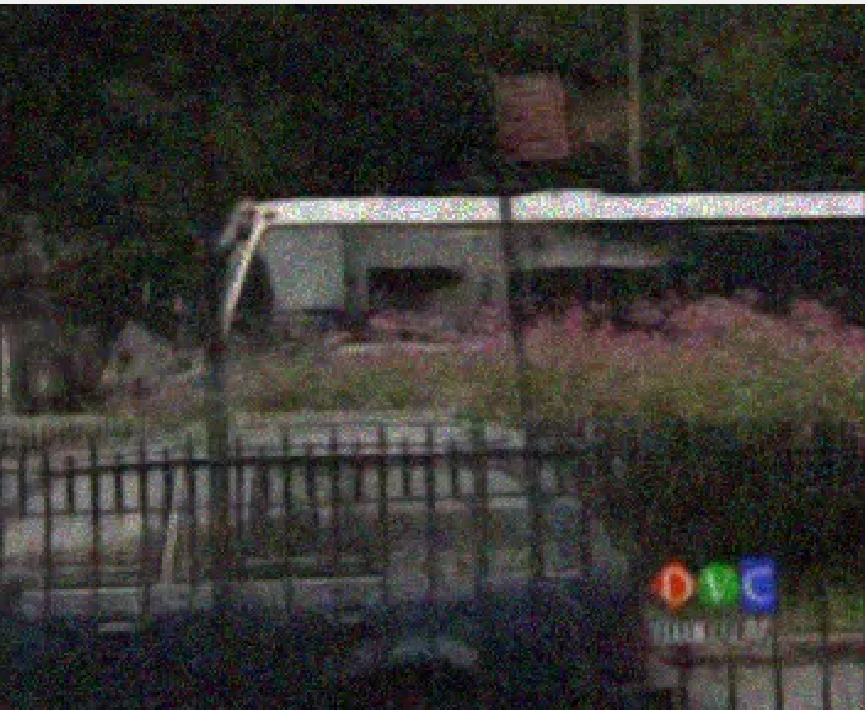
\includegraphics[width=\linewidth]{Images/Bus_1_denoised.png}
        \caption{Result of Low rank matrix completion based denoising}
    \end{minipage}
\end{figure}
\\
\textbf{PSNR obtained}

% Make table
\begin{table}[H]
    \begin{tabular}{|c|c|c|}
    \hline
    \textbf{ }     & Median Filtered Video & Denoised Video  \\
    \hline
    \textbf{PSNR} & 14.778935             & 17.714321   \\ 
    \hline
\end{tabular}
\end{table}

\newpage
\subsubsection*{Poisson dominated noise}
The noise parameters used are: \\
\begin{itemize}
    \item $\sigma = 10$
    \item $\kappa = 25$
    \item $s = 0.2$
\end{itemize}

\begin{figure}[H]
    \centering
    \begin{minipage}{.45\textwidth}
        \centering
        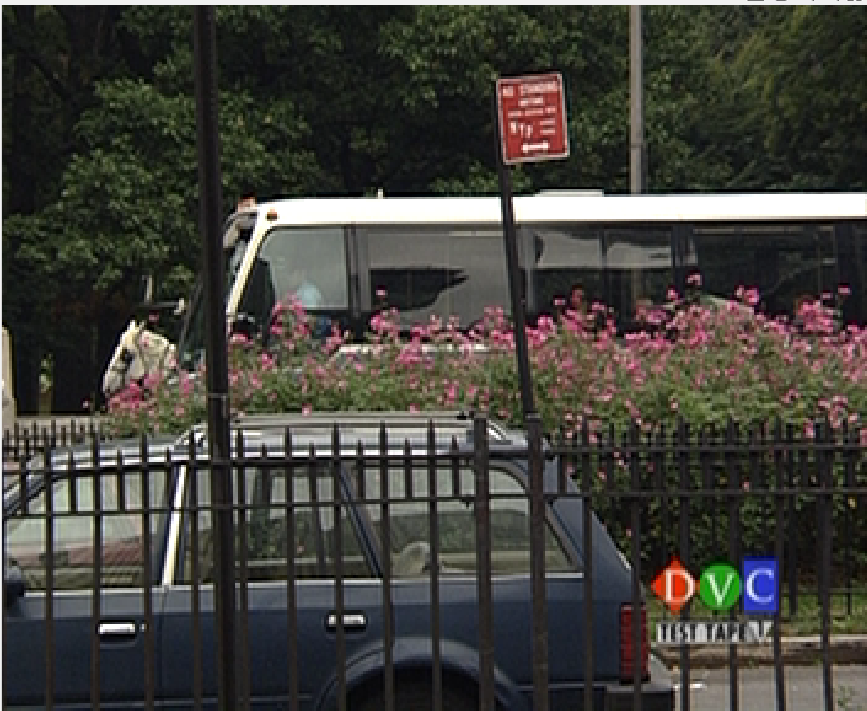
\includegraphics[width=\linewidth]{Images/Bus_original.png}
        \caption{Original Video frame}
        \label{fig:totalpowervst}
    \end{minipage}
    \begin{minipage}{.45\textwidth}
        \centering
        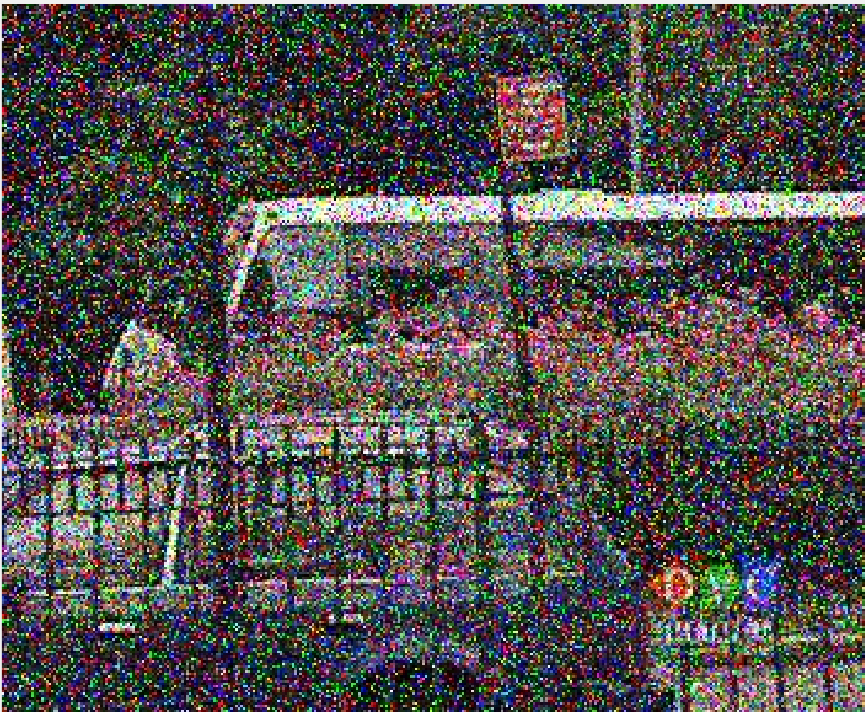
\includegraphics[width=\linewidth]{Images/Bus_2_noisy.png}
        \caption{Noisy Video frame}
    \end{minipage}
\end{figure}

\begin{figure}[H]
    \centering
    \begin{minipage}{.45\textwidth}
        \centering
        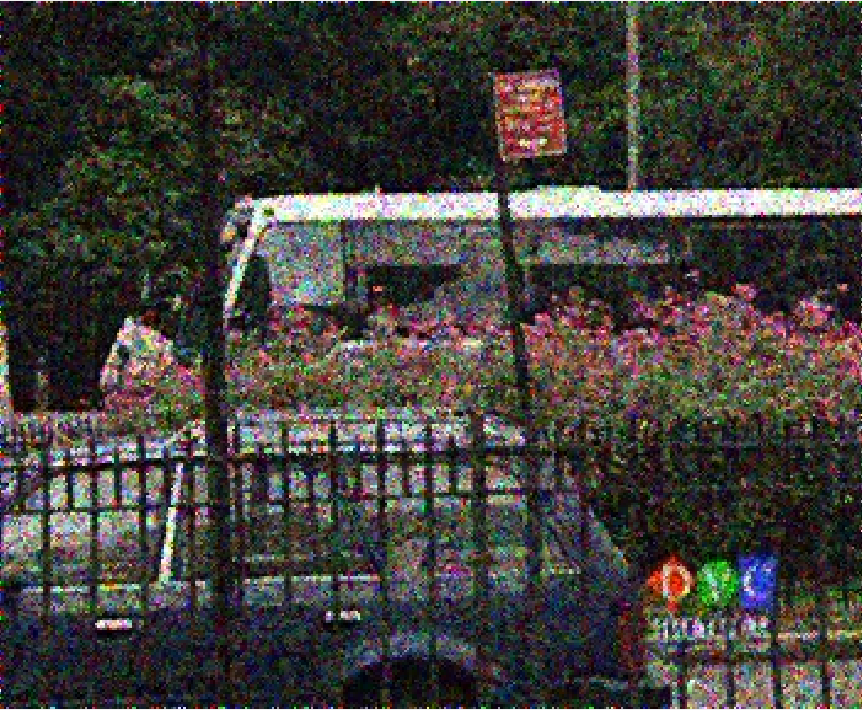
\includegraphics[width=\linewidth]{Images/Bus_2_median_filter.png}
        \caption{Result of Median Filtering}
    \end{minipage}
    \begin{minipage}{.45\textwidth}
        \centering
        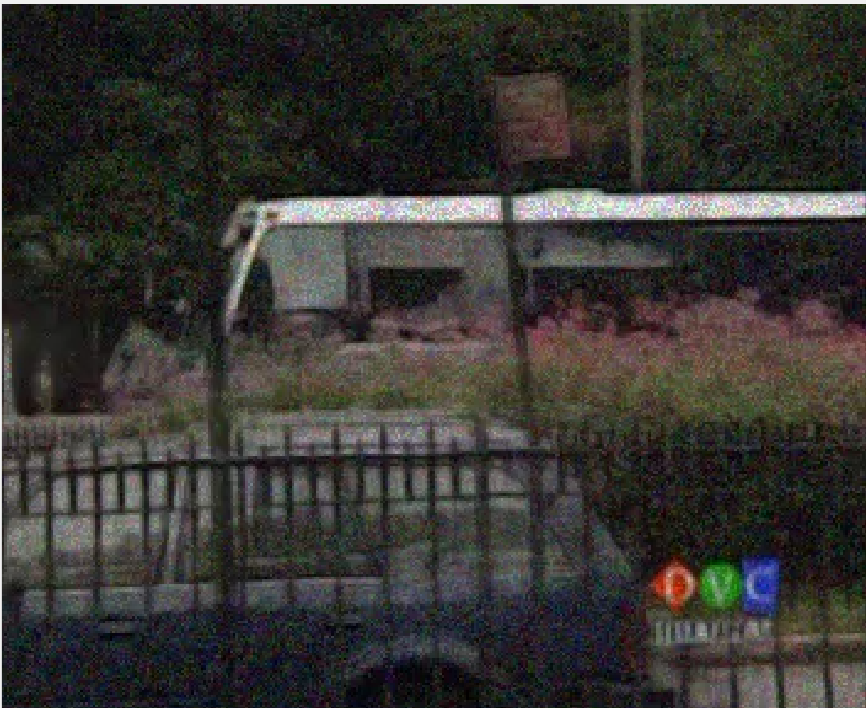
\includegraphics[width=\linewidth]{Images/Bus_2_denoised.png}
        \caption{Result of Low rank matrix completion based denoising}
    \end{minipage}
\end{figure}

\textbf{PSNR obtained}
\begin{table}[H]
    \begin{tabular}{|c|c|c|}
    \hline
    \textbf{}     & Median Filtered Video & Denoised Video   \\
    \hline
    \textbf{PSNR} & 16.810517             & 18.123166       \\
    \hline
    \end{tabular}
    \end{table}

\newpage
\subsection{Coastguard Data}
\subsubsection*{Gaussian dominated noise}
The noise parameters used are: \\
\begin{itemize}
    \item $\sigma = 50$
    \item $\kappa = 15$
    \item $s = 0.2$
\end{itemize}

\begin{figure}[H]
    \centering
    \begin{minipage}{.45\textwidth}
        \centering
        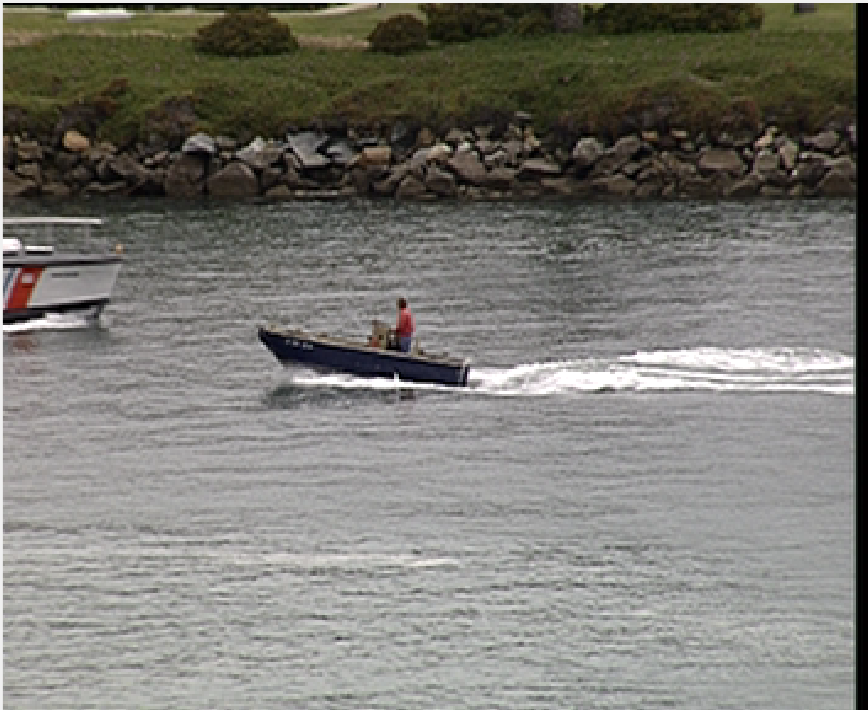
\includegraphics[width=\linewidth]{Images/Coastguard_original.png}
        \caption{Original Video frame}
        \label{fig:totalpowervst}
    \end{minipage}
    \begin{minipage}{.45\textwidth}
        \centering
        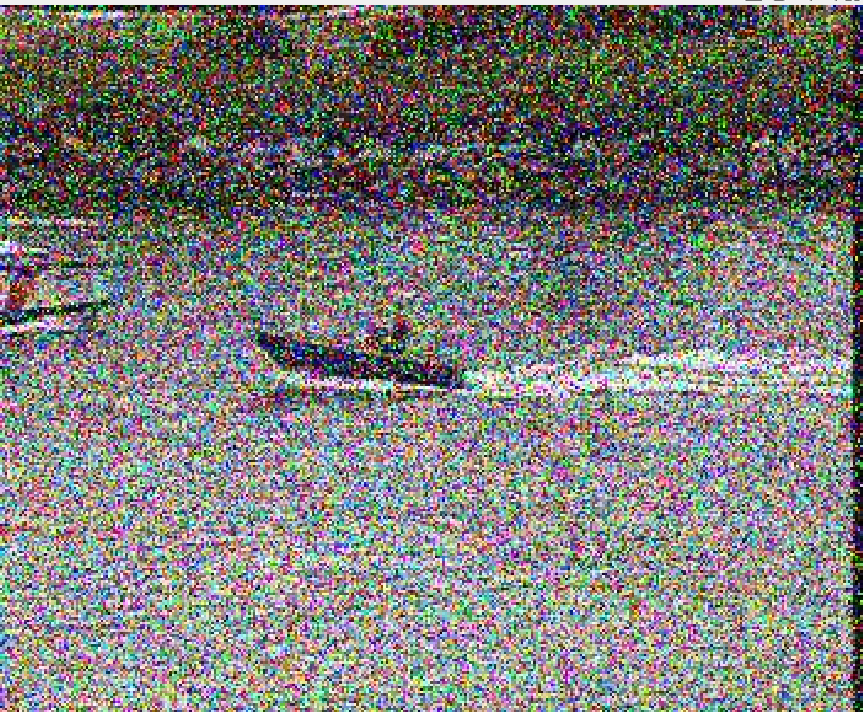
\includegraphics[width=\linewidth]{Images/Coastguard_1_noisy.png}
        \caption{Noisy Video frame}
    \end{minipage}
\end{figure}

\begin{figure}[H]
    \centering
    \begin{minipage}{.45\textwidth}
        \centering
        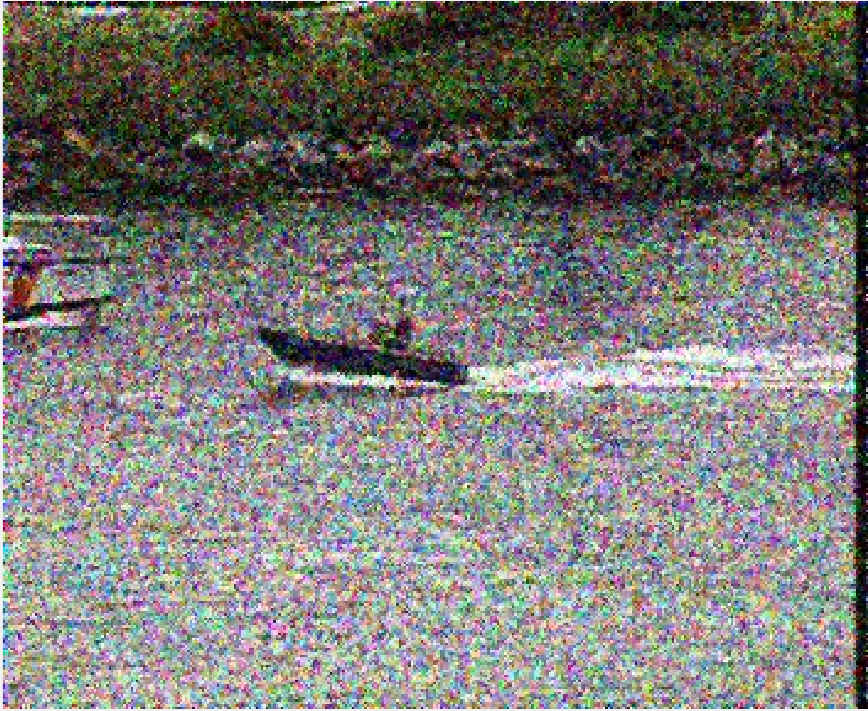
\includegraphics[width=\linewidth]{Images/Coastguard_1_median_filter.png}
        \caption{Result of Median Filtering}
    \end{minipage}
    \begin{minipage}{.45\textwidth}
        \centering
        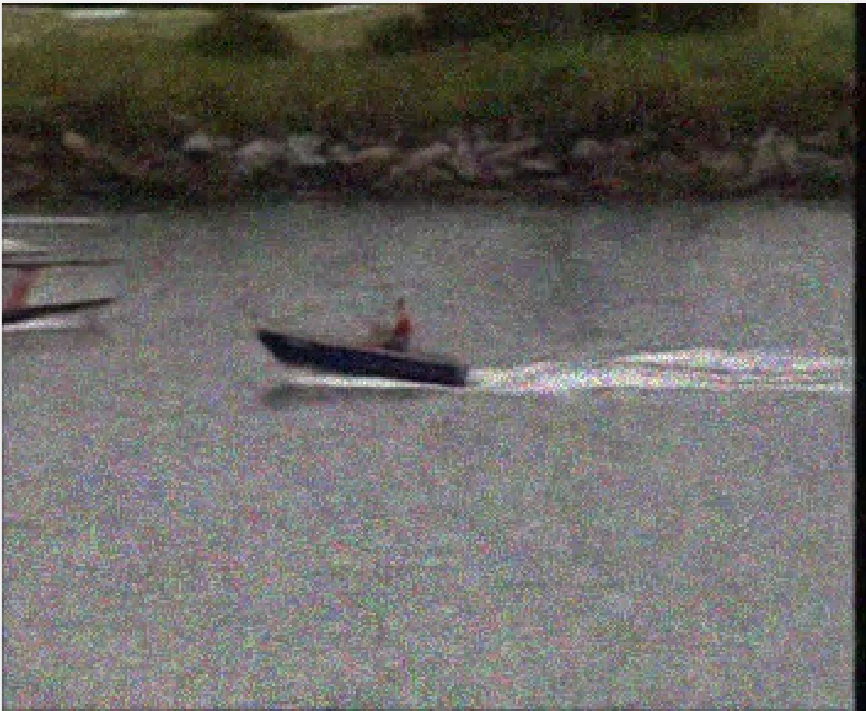
\includegraphics[width=\linewidth]{Images/Coastguard_1_denoised.png}
        \caption{Result of Low rank matrix completion based denoising}
    \end{minipage}
\end{figure}

\textbf{PSNR obtained}
\begin{table}[H]
    \begin{tabular}{|c|c|c|}
    \hline
    \textbf{}     & Median Filtered Video & Denoised Video   \\
    \hline
    \textbf{PSNR} & 13.725386             & 17.662017      \\ 
    \hline
    \end{tabular}
    \end{table}

\newpage
\subsubsection*{Poisson dominated noise}
The noise parameters used are: \\
\begin{itemize}
    \item $\sigma = 10$
    \item $\kappa = 25$
    \item $s = 0.2$
\end{itemize}

\begin{figure}[H]
    \centering
    \begin{minipage}{.45\textwidth}
        \centering
        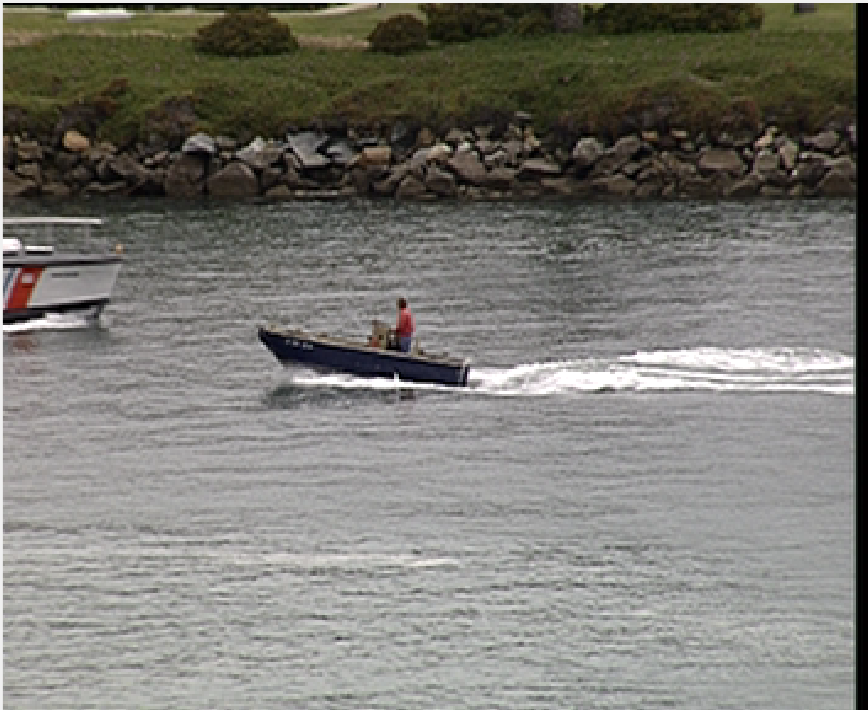
\includegraphics[width=\linewidth]{Images/Coastguard_original.png}
        \caption{Original Video frame}
        \label{fig:totalpowervst}
    \end{minipage}
    \begin{minipage}{.45\textwidth}
        \centering
        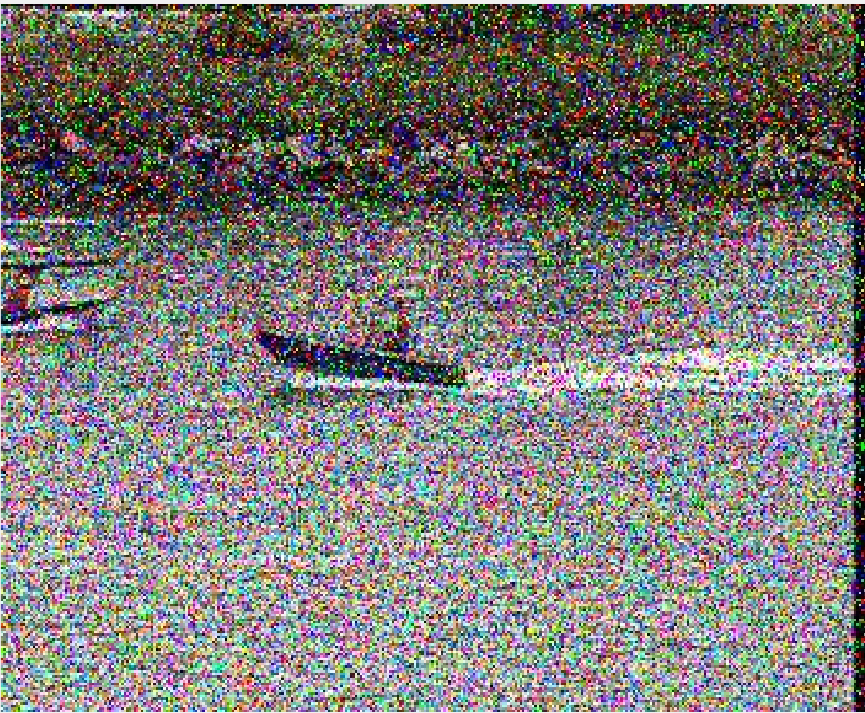
\includegraphics[width=\linewidth]{Images/Coastguard_2_noisy.png}
        \caption{Noisy Video frame}
    \end{minipage}
\end{figure}

\begin{figure}[H]
    \centering
    \begin{minipage}{.45\textwidth}
        \centering
        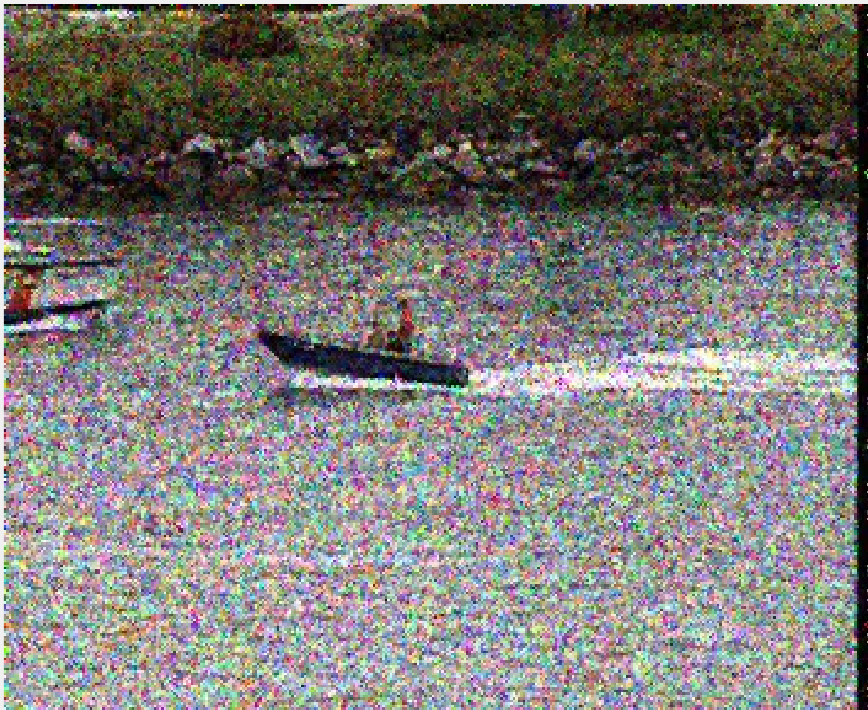
\includegraphics[width=\linewidth]{Images/Coastguard_2_median_filter.png}
        \caption{Result of Median Filtering}
    \end{minipage}
    \begin{minipage}{.45\textwidth}
        \centering
        % 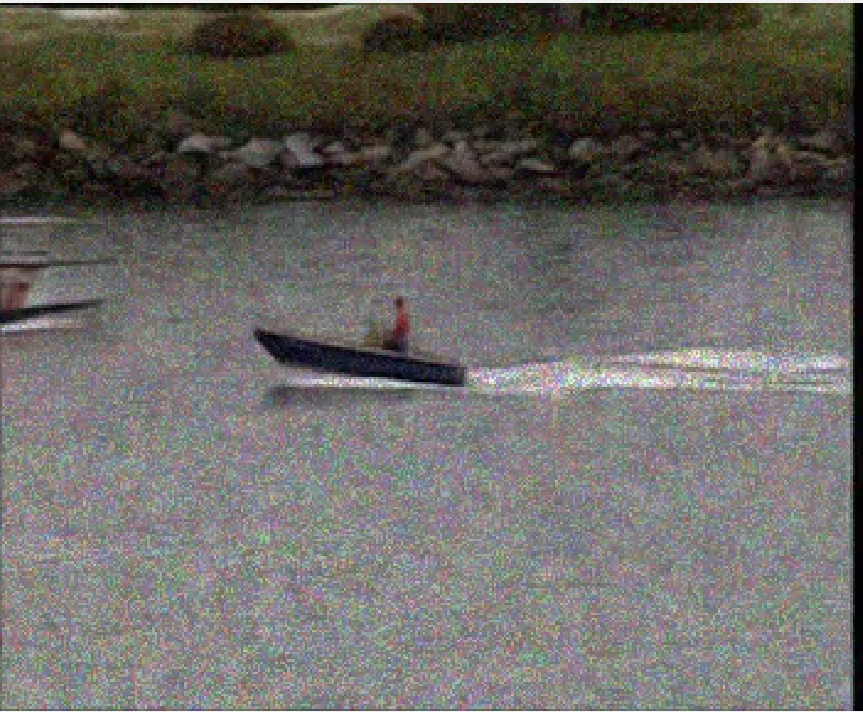
\includegraphics[width=\linewidth]{Images/Coastguard_2_denoised.png}
        \caption{Result of Low rank matrix completion based denoising}
    \end{minipage}
\end{figure}

\textbf{PSNR obtained}
\begin{table}[H]
    \begin{tabular}{|c|c|c|}
    \hline
    \textbf{}     & Median Filtered Video & Denoised Video   \\
    \hline
    \textbf{PSNR} &          14.853915             &     18.298105           \\ 
    \hline
    \end{tabular}
    \end{table}

\newpage
\subsubsection*{Additional experiments results}
These experiments are performed only on the 'Bus' dataset. For these experiments $\sigma$ is set to $10$, while $\kappa$ and $s$ are varied. The PSNR values are shown in the table below.

\textbf{Noisy Image}
\begin{table}[H]
    \begin{tabular}{|c|c|c|}
    \hline
    $ s \setminus \kappa$ & \textbf{5} & \textbf{30} \\
    \hline
    \textbf{0.1}          & 13.904347  & 12.394207    \\
    \hline
    \textbf{0.4}          & 8.408727  & 8.078162   \\
    \hline
    \end{tabular}
    \end{table}


\textbf{Median Filtering Results}
\begin{table}[H]
    \begin{tabular}{|c|c|c|}
    \hline
    $ s \setminus \kappa$ & \textbf{5} & \textbf{30} \\
    \hline
    \textbf{0.1}          & 21.433366  & 16.855396   \\
    \hline
    \textbf{0.4}          & 18.306597  & 14.907927 \\
    \hline
    \end{tabular}
    \end{table}

\texbf{Denoised Image Results}
\begin{table}[H]
    \begin{tabular}{|c|c|c|}
    \hline
    $ s \setminus \kappa$ & \textbf{5} & \textbf{30} \\
    \hline
    \textbf{0.1}          & 21.636790  & 18.909378   \\
    \hline
    \textbf{0.4}          & 19.492610  & 17.170433  \\
    \hline
    \end{tabular}
    \end{table}


\section{Observations}

\begin{itemize}
    \item The denoising algorithm performs a lot better than basic techniques like adaptive median filtering. 
    \item The algorithm is robust to mixed noise and thus give its best performance on various types of noise like gaussian, poisson, and impulsive. 
    \item 
\end{itemize}

\begin{thebibliography}{}
\bibitem{H Ji} H. Ji, C. Liu, Z. Shen and Y. Xu, "Robust video denoising using low rank matrix completion," 2010 IEEE Computer Society Conference on Computer Vision and Pattern Recognition, 2010, pp. 1791-1798, doi: 10.1109/CVPR.2010.5539849.

\bibitem{median} H. Hwang and R. A. Haddad. Adaptive median filters: New algorithms and results. IEEE Trans. on Image Processing,
4:499–502, 1995.

\bibitem{svt} S. Ma, D. goldfarb, and Z.Wan. Fixed point and bregman iterative methods for matrix rank minimization. Mathematical
Programming Series A, To appear, 2009.

\bibitem{data} Dataset source url=”http://media.xiph.org/video/derf/”.

\end{thebibliography}

\end{document}
